%----------------------------------------------------------------------------------------
%	PACKAGES AND OTHER DOCUMENT CONFIGURATIONS
%----------------------------------------------------------------------------------------

\documentclass{article}

\usepackage{fancyhdr} % Required for custom headers
\usepackage{lastpage} % Required to determine the last page for the footer
\usepackage{extramarks} % Required for headers and footers
\usepackage{graphicx} % Required to insert images
\usepackage{lipsum} % Used for inserting dummy 'Lorem ipsum' text into the template
\usepackage{parskip}
\usepackage{url}
\usepackage{float}
\usepackage{booktabs} % Horizontal rules in tables
\usepackage{setspace}
\usepackage{pdfpages}
\usepackage{fourier}
\usepackage[small,compact]{titlesec}

% Margins
\topmargin=-0.5in
\evensidemargin=0in
\oddsidemargin=0in
\textwidth=6.0in
\textheight=9.0in
\headsep=0.2in 

% Set up the header and footer
\pagestyle{fancy}
\chead{} % Top center header
\rhead{\firstxmark} % Top right header
\lfoot{\lastxmark} % Bottom left footer
\cfoot{} % Bottom center footer
\rfoot{Page\ \thepage\ of\ \pageref{LastPage}} % Bottom right footer
\renewcommand\headrulewidth{0.4pt} % Size of the header rule
\renewcommand\footrulewidth{0.4pt} % Size of the footer rule

\setlength\parindent{0pt} % Removes all indentation from paragraphs

%----------------------------------------------------------------------------------------
%	DOCUMENT STRUCTURE COMMANDS
%	Skip this unless you know what you're doing
%----------------------------------------------------------------------------------------

% Header and footer for when a page split occurs within a section
\newcommand{\enterSectionHeader}[1]{
\nobreak\extramarks{}{}\nobreak
\nobreak\extramarks{}{}\nobreak
}

\setcounter{secnumdepth}{0} % Removes default section numbers
\newcounter{docSectionCounter} % Creates a counter to keep track of the number of sections

\newcommand{\docSectionName}{}
\newenvironment{docSection}[1][Section \arabic{docSectionCounter}]{ % Makes a new environment called docSection which takes 1 argument (custom name) but the default is "Section #"
\stepcounter{docSectionCounter} % Increase counter for number of sections
\renewcommand{\docSectionName}{#1} % Assign \docSectionName the name of the section
\section{\docSectionName} % Make a section in the document with the custom section count
\enterSectionHeader{\docSectionName} % Header and footer within the environment
}{
}

\newcommand{\noteBox}[1]{ % Defines the notebox command with the content as the only argument
\vspace{10pt}\noindent\framebox[\columnwidth][c]{\begin{minipage}{0.98\columnwidth}\textbf{NOTE }#1\end{minipage}} % Makes the box around the note and puts the content inside
}

\newcommand{\docSubsectionName}{}
\newenvironment{docSubsection}[1]{ % New environment for sections within doc problems, takes 1 argument - the name of the section
\renewcommand{\docSubsectionName}{#1} % Assign \docSubsectionName to the name of the section from the environment argument
\subsection{\docSubsectionName} % Make a subsection with the custom name of the subsection
\enterSectionHeader{\docSubsectionName} % Header and footer within the environment
}{
\enterSectionHeader{\docSectionName} % Header and footer after the environment
}
   
%----------------------------------------------------------------------------------------
%	NAME AND CLASS SECTION
%----------------------------------------------------------------------------------------

\newcommand{\docTitle}{Faun: A Lightweight IMAP Mail Client} % Document title
\newcommand{\docDate}{Monday,\ April\ 8,\ 2013} % Date
\newcommand{\docClass}{CSCI3171: Network Computing} % Course/class
\newcommand{\docClassInstructor}{--- Project ---} % Teacher/lecturer
\newcommand{\docAuthorName}{Alex Safatli} % Your name

%----------------------------------------------------------------------------------------
%	TITLE PAGE
%----------------------------------------------------------------------------------------

\title{
\vspace{2in}
\textmd{\textbf{\docClass}}\\
\textmd{\docTitle}\\
\vspace{0.1in}\large{\textit{\docClassInstructor}}\\
\vspace{3in}
}

\author{\textbf{\docAuthorName}}
\date{\docDate}

%----------------------------------------------------------------------------------------

\begin{document}

\maketitle
\newpage
\tableofcontents
\newpage
\onehalfspace

%----------------------------------------------------------------------------------------
%	CONTENT
%----------------------------------------------------------------------------------------

% Use \clearpage to page break.

\begin{docSection}[Problem Overview]
\begin{docSubsection}{Problem Description}
The purpose of this project is to implement a Internet Message Access Protocol (\textbf{IMAP}) interface to provide functionality that builds on but hides the protocol. The following was desired to be manifested in this interface:

\begin{itemize}
    \item as many functions as possible would be implemented from the prescribed \textbf{IMAP 4rev1} request for comments (\textbf{RFC}),
    \item as little as possible use of outside libraries; most of the functionality will be derived from base socket communications,
    \item the handling of communication with any SMTP-enabled \textbf{mail server} that accepts IMAP messages, and
    \item secure communication of credentials, preferably through a Secure Sockets Layer (\textbf{SSL}).
\end{itemize}

In order to serve the comforts of the programmer, this would preferably be programmed in \textbf{Python}.
\end{docSubsection}

\begin{docSubsection}{Solution}
The solution that came about is a Python program designed as a text-based mail retrieval solution in order to contact a specified hostname for a mail server at a specified port number (this would be typically 993 for SSL-communication or 143 for typical IMAP communication).

This program is entitled \textbf{Faun}. The origin of the name is from the film \textit{Pan's Labyrinth}, sometimes known by its Spanish name \textit{El Laberinto del Fauno} (the Labyrinth of the Faun). As a Faun is typically a mythical servant, this seemed like a fitting name for a client designed to serve as a mail retrieval client.
\end{docSubsection}

\end{docSection}

\begin{docSection}[Design]
\begin{docSubsection}{Classes and Code Structure}

Two files with code in them are present in order to comprise the program that was created in order to represent two different modules, both key to the functionality of this program:

\begin{enumerate}
    \item \texttt{faun.py}: encompasses the working program; will possess flags in order to specify parameters including the hostname of the computer to connect to a port number, and a username. Furthermore, the function of this client will be to ask the user for further instruction after initiating a connection with the mail server.
    \item \texttt{dispatcher.py}: encompasses all stream/socket communication functions in one module so as to encapsulate and hide this information from other elements of the program. In this regard, it takes control and manages format of messages, what actions to take when messages are received, and handles these in the order in which they are received. Messages are also saved by identifying tag for organization.
\end{enumerate}

\begin{figure}[h]
\centering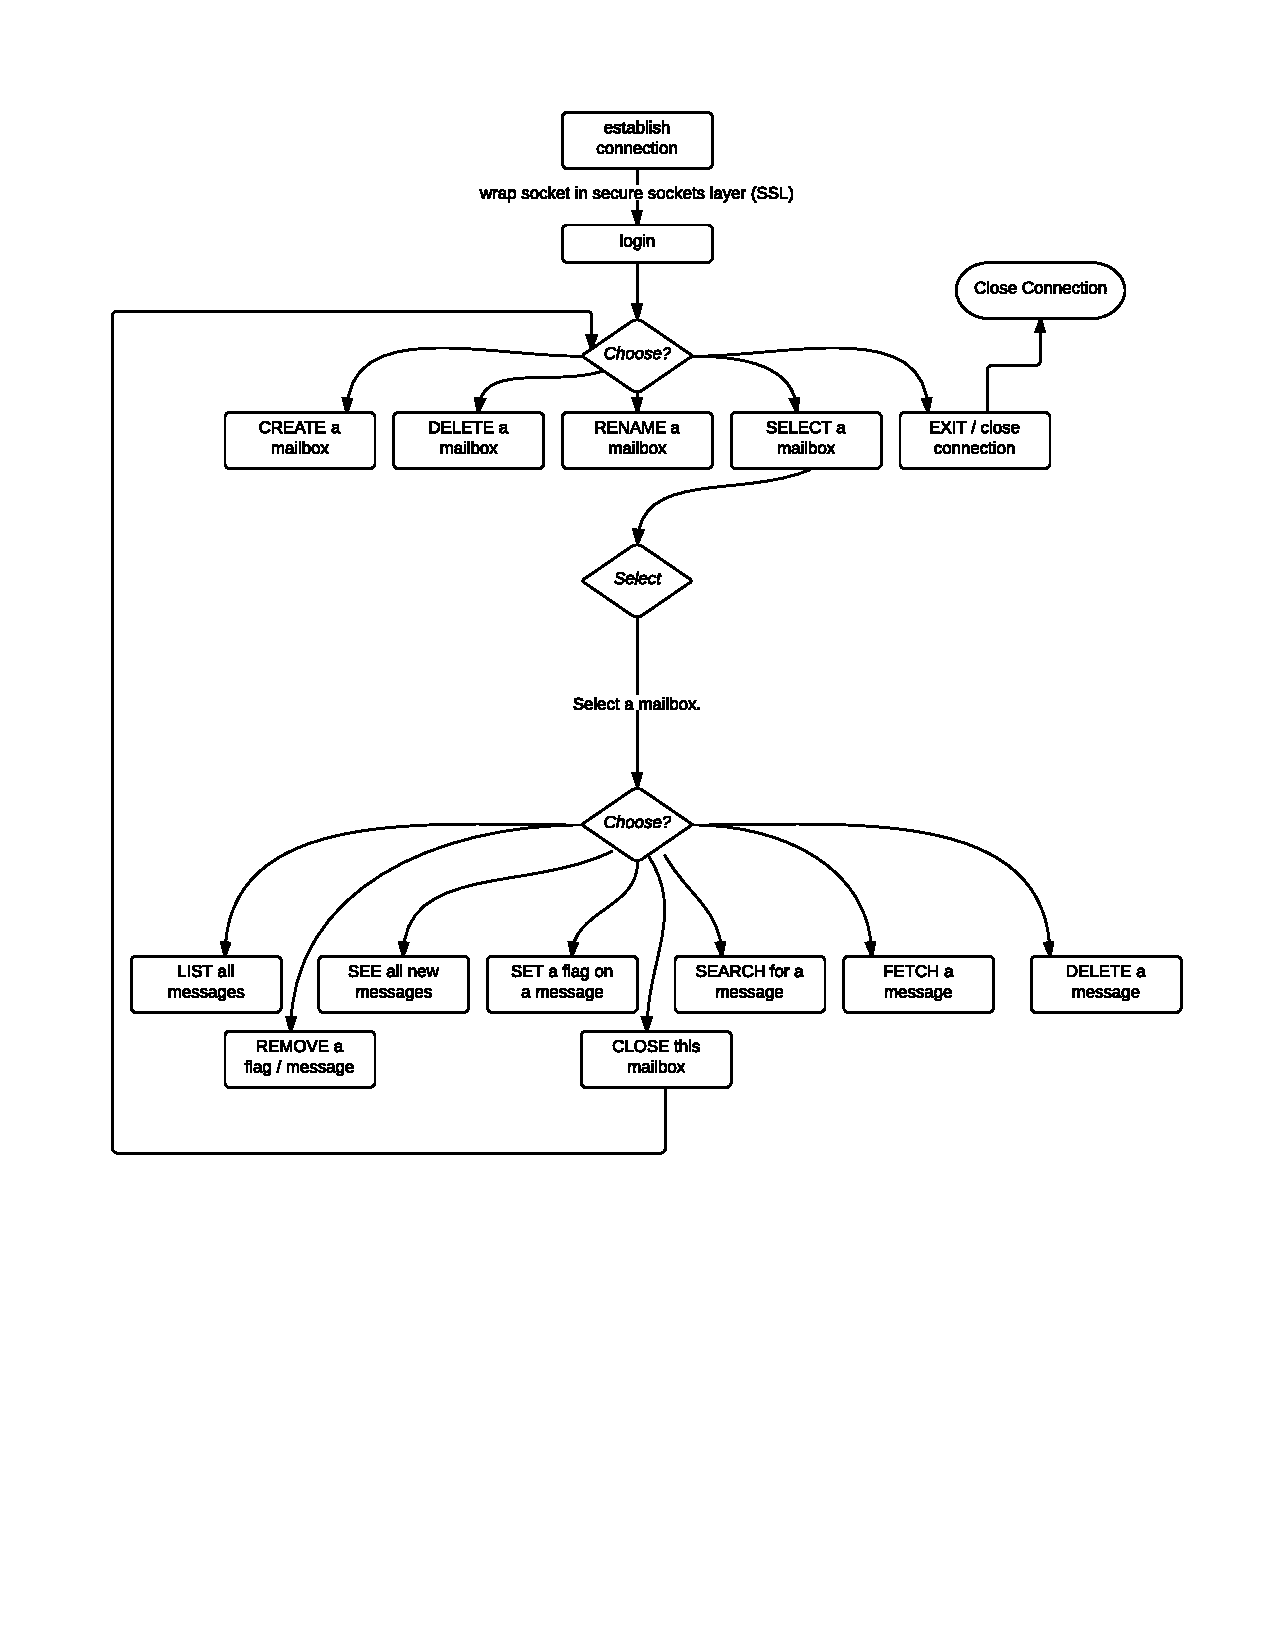
\includegraphics[width=1.0\textwidth]{flowchart.pdf}
\caption{\textit{A small flowchart representing the function of the main program.}}
\end{figure}

The \texttt{faun.py} file contains class \texttt{mail\_box}, which is a small helper class equivalent to a C \texttt{struct} in order to manage information about mailboxes, and several functions. The \texttt{dispatch.py} file contains classes \texttt{dispatcher}, \texttt{tag} that manages the identifier tag present in low-level IMAP messages, and \texttt{response}/\texttt{request} message class definitions for respective responses and request messages from and to the server.

As it can be shown in \textbf{Figure 1}, most of the functions underlined in RFC3501 for the IMAP 4rev1 protocol are covered by the main program; the only ones not covered include the \texttt{NOOP}, \texttt{SUBSCRIBE} and its corresponding functions, \texttt{LSUB}, \texttt{STATUS}, \texttt{APPEND}, \texttt{CHECK}, \texttt{UID} and \texttt{EXPUNGE} commands. Most of these were implemented for reasons of either possessing on reason to or because there did not seem a practical reason to implement it in a mail client of \textbf{Faun}'s nature.

\begin{itemize}
    \item \texttt{NOOP}; a command that does nothing, 
    \item \texttt{SUBSCRIBE} and its corresponding functions, including \texttt{LSUB} which provide very little in terms of functionality to a user, 
    \item \texttt{STATUS}; only allows investigation of other mailboxes outside of a selected one, 
    \item \texttt{APPEND}; mail delivery is not possible with solely \textbf{IMAP} and therefore there was no need to provide the implementation of this element of the protocol --- SMTP is also necessary in order to provide this functionality, 
    \item \texttt{CHECK}; an implementation-specific command for housekeeping,
    \item \texttt{UID}; a useful utility command that was not used in this implementation, and 
    \item \texttt{EXPUNGE}; permanently deletes all messages flagged as deleted, but deletion is managed when a mailbox is closed.
\end{itemize}

\end{docSubsection}
\begin{docSubsection}{Function}
In order to use the program, run the \textbf{main program} by either calling \texttt{python faun.py} or \texttt{./faun.py} if the file has execution permissions and a bash shell is used, with \texttt{.} replaced with the directory of the file or left as is if in the directory where the file is. 

The designation of host name and port number can be made through command-line flags. In order to see all possible options, type in the following to bring up a help menu:

\begin{verbatim} 
python faun.py -h
\end{verbatim}

\end{docSubsection}

\begin{docSubsection}{Data Structures}
For the most part, a dictionary was used to store tag-message pairs within the dispatcher along with strings to denote respective protocol name, version number, path, parameters, and operations (see \texttt{dispatcher.py}). 

Linked lists, implemented as a built-in list, are used to store the contents of consecutive information messages from the server that denotes longer bodies including mail messages, mailbox lists, and lists of messages.
\end{docSubsection}
\end{docSection}
\begin{docSection}[Analysis]
\begin{docSubsection}{Results}
The mail client, \textbf{Faun}, that was created for this project performs many simple mail tasks and even allow users to output mail messages to external files. For the most part, this client will allow straight-forward and cursory investigation of a mail server and mail messages on that server where, unless the user wishes it, nothing is disturbed on the server.

Utilizing base-level socket communication, the IMAP protocol was mostly made functional and an interface, through the \textbf{Faun} program, is provided in order to mask this low-level string processing.

A sample run of the program is included below.

\begin{verbatim}
python faun.py -s fcspostoffice.cs.dal.ca
>> Username: safatli
>> Password: 

Securely logged in as safatli on hostname fcspostoffice.cs.dal.ca.

What would you like to do?
  0. CREATE a mailbox
  1. DELETE a mailbox
  2. RENAME a mailbox
  3. SELECT a mailbox
  4. EXIT and close connection
>> Choose an option: 3

5 mailboxes were found on the server.
  0. INBOX
  1. Drafts
  2. Junk
  3. Sent
  4. Trash
>> Select a mailbox: 0

32 messages in mailbox.
0 recent messages found.

Mailbox: INBOX; specify what to do next:
  0. LIST all messages
  1. SEE all new messages
  2. SET a flag on a message
  3. SEARCH for a message
  4. FETCH a message
  5. DELETE a message
  6. REMOVE a flag from a message
  7. CLOSE this mailbox
>> Choose an option: 3
>> Search for: car

Showing 10 messages at a time (of 3)...
  5. Subject: CSUGRADS> Career Conversations Starting Wednesday, Jan 12 11:30am
  11. Subject: CSUGRADS> Reminder - Career Conversations today 11:30 Room 430
  16. Subject: Assignment 2

Mailbox: INBOX; specify what to do next:
  0. LIST all messages
  1. SEE all new messages
  2. SET a flag on a message
  3. SEARCH for a message
  4. FETCH a message
  5. DELETE a message
  6. REMOVE a flag from a message
  7. CLOSE this mailbox
>> Choose an option: 4
>> Specify message UID (or b to return): 16

--- Begin message 16 ---
Date: Tue, 1 Feb 2011 00:16:16 -0400
Subject: Assignment 2
From: "Nauzer Kalyaniwalla" <nauzerk@cs.dal.ca>
To: all-cs2112@cs.dal.ca


 Hello All,

 Assignment 2 is available on the course web-page:

 http://www.cs.dal.ca/~nauzerk/discrete

 Please look it over carefully  before the next class.

 Nauzer


Faculty of Computer Science
Dalhousie University
Halifax NS
B3H-1W5
(902)-494-2841

--- End message 16 ---
Save e-mail to file (y/n)? n

Mailbox: INBOX; specify what to do next:
  0. LIST all messages
  1. SEE all new messages
  2. SET a flag on a message
  3. SEARCH for a message
  4. FETCH a message
  5. DELETE a message
  6. REMOVE a flag from a message
  7. CLOSE this mailbox
>> Choose an option: 7

What would you like to do?
  0. CREATE a mailbox
  1. DELETE a mailbox
  2. RENAME a mailbox
  3. SELECT a mailbox
  4. EXIT and close connection
>> Choose an option: 4
\end{verbatim}

\end{docSubsection}
\begin{docSubsection}{Strengths and Weaknesses}
All of the protocol elements investigated are strongly represented in a text-based format. However, very little manipulation of messages (including replying to messages, forwarding messages, and composing messages) is possible because of the nature of the IMAP protocol: it has no method or technique that allows for the delivery of messages.

In hindsight, a better way to have implemented this program would have been utilizing a \textbf{Graphical User Interface} (GUI) as well as implementing the appropriately functionality of SMTP communication in order to compose messages (this would be paired with the \texttt{APPEND} function above in order to append sent messages to an appropriate \texttt{sent-mail} mailbox).

The graphical user interface would have included a single column for listing messages in a given mailbox and then another portion of the window to present messages.
\end{docSubsection}


\end{docSection}
\end{document}
